% Options for packages loaded elsewhere
\PassOptionsToPackage{unicode}{hyperref}
\PassOptionsToPackage{hyphens}{url}
%
\documentclass[
]{article}
\usepackage{amsmath,amssymb}
\usepackage{iftex}
\ifPDFTeX
  \usepackage[T1]{fontenc}
  \usepackage[utf8]{inputenc}
  \usepackage{textcomp} % provide euro and other symbols
\else % if luatex or xetex
  \usepackage{unicode-math} % this also loads fontspec
  \defaultfontfeatures{Scale=MatchLowercase}
  \defaultfontfeatures[\rmfamily]{Ligatures=TeX,Scale=1}
\fi
\usepackage{lmodern}
\ifPDFTeX\else
  % xetex/luatex font selection
\fi
% Use upquote if available, for straight quotes in verbatim environments
\IfFileExists{upquote.sty}{\usepackage{upquote}}{}
\IfFileExists{microtype.sty}{% use microtype if available
  \usepackage[]{microtype}
  \UseMicrotypeSet[protrusion]{basicmath} % disable protrusion for tt fonts
}{}
\makeatletter
\@ifundefined{KOMAClassName}{% if non-KOMA class
  \IfFileExists{parskip.sty}{%
    \usepackage{parskip}
  }{% else
    \setlength{\parindent}{0pt}
    \setlength{\parskip}{6pt plus 2pt minus 1pt}}
}{% if KOMA class
  \KOMAoptions{parskip=half}}
\makeatother
\usepackage{xcolor}
\usepackage[margin=1in]{geometry}
\usepackage{color}
\usepackage{fancyvrb}
\newcommand{\VerbBar}{|}
\newcommand{\VERB}{\Verb[commandchars=\\\{\}]}
\DefineVerbatimEnvironment{Highlighting}{Verbatim}{commandchars=\\\{\}}
% Add ',fontsize=\small' for more characters per line
\usepackage{framed}
\definecolor{shadecolor}{RGB}{248,248,248}
\newenvironment{Shaded}{\begin{snugshade}}{\end{snugshade}}
\newcommand{\AlertTok}[1]{\textcolor[rgb]{0.94,0.16,0.16}{#1}}
\newcommand{\AnnotationTok}[1]{\textcolor[rgb]{0.56,0.35,0.01}{\textbf{\textit{#1}}}}
\newcommand{\AttributeTok}[1]{\textcolor[rgb]{0.13,0.29,0.53}{#1}}
\newcommand{\BaseNTok}[1]{\textcolor[rgb]{0.00,0.00,0.81}{#1}}
\newcommand{\BuiltInTok}[1]{#1}
\newcommand{\CharTok}[1]{\textcolor[rgb]{0.31,0.60,0.02}{#1}}
\newcommand{\CommentTok}[1]{\textcolor[rgb]{0.56,0.35,0.01}{\textit{#1}}}
\newcommand{\CommentVarTok}[1]{\textcolor[rgb]{0.56,0.35,0.01}{\textbf{\textit{#1}}}}
\newcommand{\ConstantTok}[1]{\textcolor[rgb]{0.56,0.35,0.01}{#1}}
\newcommand{\ControlFlowTok}[1]{\textcolor[rgb]{0.13,0.29,0.53}{\textbf{#1}}}
\newcommand{\DataTypeTok}[1]{\textcolor[rgb]{0.13,0.29,0.53}{#1}}
\newcommand{\DecValTok}[1]{\textcolor[rgb]{0.00,0.00,0.81}{#1}}
\newcommand{\DocumentationTok}[1]{\textcolor[rgb]{0.56,0.35,0.01}{\textbf{\textit{#1}}}}
\newcommand{\ErrorTok}[1]{\textcolor[rgb]{0.64,0.00,0.00}{\textbf{#1}}}
\newcommand{\ExtensionTok}[1]{#1}
\newcommand{\FloatTok}[1]{\textcolor[rgb]{0.00,0.00,0.81}{#1}}
\newcommand{\FunctionTok}[1]{\textcolor[rgb]{0.13,0.29,0.53}{\textbf{#1}}}
\newcommand{\ImportTok}[1]{#1}
\newcommand{\InformationTok}[1]{\textcolor[rgb]{0.56,0.35,0.01}{\textbf{\textit{#1}}}}
\newcommand{\KeywordTok}[1]{\textcolor[rgb]{0.13,0.29,0.53}{\textbf{#1}}}
\newcommand{\NormalTok}[1]{#1}
\newcommand{\OperatorTok}[1]{\textcolor[rgb]{0.81,0.36,0.00}{\textbf{#1}}}
\newcommand{\OtherTok}[1]{\textcolor[rgb]{0.56,0.35,0.01}{#1}}
\newcommand{\PreprocessorTok}[1]{\textcolor[rgb]{0.56,0.35,0.01}{\textit{#1}}}
\newcommand{\RegionMarkerTok}[1]{#1}
\newcommand{\SpecialCharTok}[1]{\textcolor[rgb]{0.81,0.36,0.00}{\textbf{#1}}}
\newcommand{\SpecialStringTok}[1]{\textcolor[rgb]{0.31,0.60,0.02}{#1}}
\newcommand{\StringTok}[1]{\textcolor[rgb]{0.31,0.60,0.02}{#1}}
\newcommand{\VariableTok}[1]{\textcolor[rgb]{0.00,0.00,0.00}{#1}}
\newcommand{\VerbatimStringTok}[1]{\textcolor[rgb]{0.31,0.60,0.02}{#1}}
\newcommand{\WarningTok}[1]{\textcolor[rgb]{0.56,0.35,0.01}{\textbf{\textit{#1}}}}
\usepackage{graphicx}
\makeatletter
\def\maxwidth{\ifdim\Gin@nat@width>\linewidth\linewidth\else\Gin@nat@width\fi}
\def\maxheight{\ifdim\Gin@nat@height>\textheight\textheight\else\Gin@nat@height\fi}
\makeatother
% Scale images if necessary, so that they will not overflow the page
% margins by default, and it is still possible to overwrite the defaults
% using explicit options in \includegraphics[width, height, ...]{}
\setkeys{Gin}{width=\maxwidth,height=\maxheight,keepaspectratio}
% Set default figure placement to htbp
\makeatletter
\def\fps@figure{htbp}
\makeatother
\setlength{\emergencystretch}{3em} % prevent overfull lines
\providecommand{\tightlist}{%
  \setlength{\itemsep}{0pt}\setlength{\parskip}{0pt}}
\setcounter{secnumdepth}{-\maxdimen} % remove section numbering
\usepackage{booktabs}
\usepackage{longtable}
\usepackage{array}
\usepackage{multirow}
\usepackage{wrapfig}
\usepackage{float}
\usepackage{colortbl}
\usepackage{pdflscape}
\usepackage{tabu}
\usepackage{threeparttable}
\usepackage{threeparttablex}
\usepackage[normalem]{ulem}
\usepackage{makecell}
\usepackage{xcolor}
\ifLuaTeX
  \usepackage{selnolig}  % disable illegal ligatures
\fi
\usepackage{bookmark}
\IfFileExists{xurl.sty}{\usepackage{xurl}}{} % add URL line breaks if available
\urlstyle{same}
\hypersetup{
  pdftitle={Demo 2: Biomedical \& Clinical Informatics},
  pdfauthor={Katherine S. Geist, PhD},
  hidelinks,
  pdfcreator={LaTeX via pandoc}}

\title{Demo 2: Biomedical \& Clinical Informatics}
\usepackage{etoolbox}
\makeatletter
\providecommand{\subtitle}[1]{% add subtitle to \maketitle
  \apptocmd{\@title}{\par {\large #1 \par}}{}{}
}
\makeatother
\subtitle{Merrimack College DSE6630: Healthcare \& Life Sciences
Analytics}
\author{Katherine S. Geist, PhD}
\date{3 June 2024}

\begin{document}
\maketitle

{
\setcounter{tocdepth}{2}
\tableofcontents
}
\section{Epidemiology of pneumonia-related hospital
readmissions}\label{epidemiology-of-pneumonia-related-hospital-readmissions}

As you work through your Project 2, keep in mind that we are actually
working with \textbf{spatial data} even though we have not focused on
that much until now. This relates to everything we will be doing in
Module 3 on Public Health \& Epidemiology, though! As data scientists of
public health and epidemiology, one of the \textbf{most powerful} tools
in our toolkit are maps.

For our hospital readmissions data, we had a lot of spatial data that we
could have leveraged but didn't really in our other analysis. This demo,
we are going to take advantage of the fact that there is a LOT of
spatial data here that we can use: \emph{addresss}, \emph{county},
\emph{state}, \emph{zip code}\ldots{} wow! We will focus first on the
\textbf{state level} data together, and then I am going to have you try
your own analysis at the county-level.

\subsection{State-level Analysis of Pneuomonia-related Hospital
Readmissions}\label{state-level-analysis-of-pneuomonia-related-hospital-readmissions}

\subsubsection{Step 1. Make a base map.}\label{step-1.-make-a-base-map.}

Let's practice bring up a very simple little map of the US from
\texttt{maps} and \texttt{ggplot2}. The \texttt{maps} package provides
latitude and longitude data for various in the package. We will do
something much more complicated for our Project 3, but for this little
exploration let's just keep it simple.

Notice that first I am having to extract state-level geographic
information from the \texttt{map\_data()} function. Similar functions
exist for other geographic levels of data, including world (country),
county, or other regions of the world.

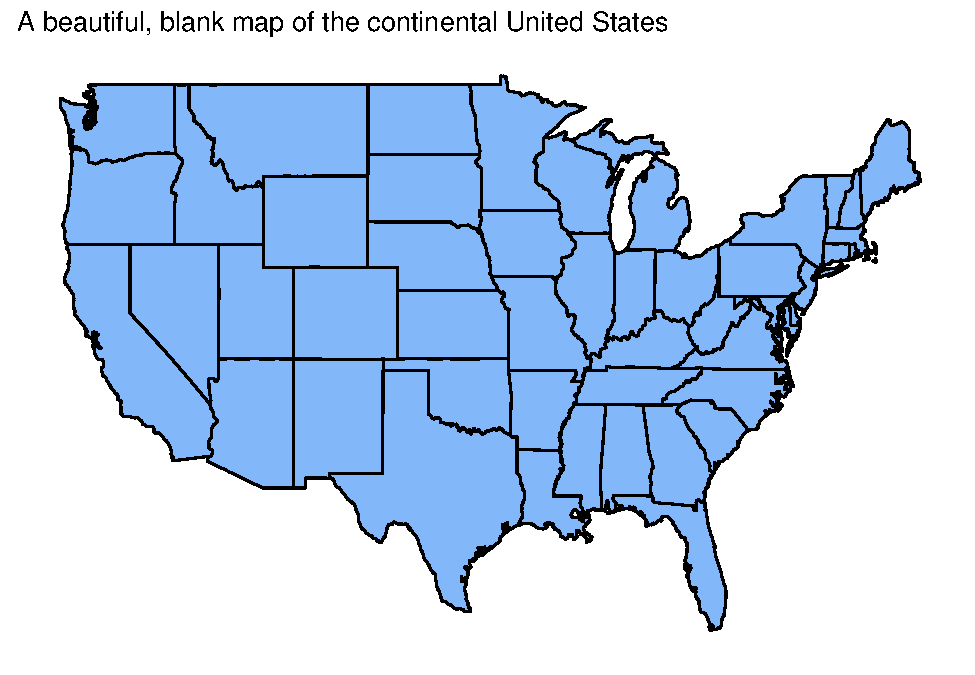
\includegraphics{Demo3_files/figure-latex/unnamed-chunk-2-1.pdf}

Great, our first map of the continental US! But it's pretty
uninteresting just as it is. Let's use this map to overlay our
pneumonia-related hospital readmissions data.

\subsubsection{Step 2. Prepare the pneumonia-related hospital
readmissions
data.}\label{step-2.-prepare-the-pneumonia-related-hospital-readmissions-data.}

Bring in the hospital readmissions data.

\begin{Shaded}
\begin{Highlighting}[]
\FunctionTok{load}\NormalTok{(}\StringTok{"../../II. Biomedical \& Clinical Informatics/Demo/pneumoniaFull.Rdata"}\NormalTok{)}
\end{Highlighting}
\end{Shaded}

Notice that I brought in our \textbf{fully merged, non-encoded,
non-transformed} dataset from Demo 2 called
\texttt{pneumoniaFull.Rdata}! Bet you didn't think you'd ever see that
again, huh?! We are using these data because they contain all our
spatial information as well as our data in the original form, which is
precisely what we would want to map.

But, before we can merge them with the state data that we extracted for
the map, notice that \texttt{State} in our pneumonia-related
readmissions data is an abbreviation (e.g., ``AL'') but it's the name of
the state in the \texttt{map\_data} (``alabama''). \textbf{How can we
fix that?}

We are going to write a function to do the mapping ourselves, but you
may wonder why. Although \texttt{maps} includes a data source,
\texttt{states.fips}, that we can load and use to get state names - the
problem there is that states with islands, like WA state or NY, can have
additional mappings that we'd miss. It's easier in this particular case
to write our own little function, I think. Notice also that I am
choosing to name the new column in \texttt{pneumoniaFull.Rdata} as
\texttt{region}; this is to match the column name in the \texttt{states}
dataframe that we use for mapping so we can join the tables more easily.

\subsubsection{\texorpdfstring{Step 3. Summarize the data by mean
\texttt{PredictedReadmissionsRate}.}{Step 3. Summarize the data by mean PredictedReadmissionsRate.}}\label{step-3.-summarize-the-data-by-mean-predictedreadmissionsrate.}

\begin{Shaded}
\begin{Highlighting}[]
\CommentTok{\# table(pneumoniaFull$State, useNA = "always")}

\NormalTok{avgReadmissions }\OtherTok{\textless{}{-}}\NormalTok{ pneumoniaFull }\SpecialCharTok{\%\textgreater{}\%} 
  \FunctionTok{select}\NormalTok{(PredictedReadmissionRate, region) }\SpecialCharTok{\%\textgreater{}\%} 
  \FunctionTok{drop\_na}\NormalTok{() }\SpecialCharTok{\%\textgreater{}\%} 
  \FunctionTok{group\_by}\NormalTok{(region) }\SpecialCharTok{\%\textgreater{}\%} 
  \FunctionTok{summarize}\NormalTok{(}\AttributeTok{avgReadmit =} \FunctionTok{mean}\NormalTok{(PredictedReadmissionRate, }\AttributeTok{na.rm =} \ConstantTok{TRUE}\NormalTok{))}

\NormalTok{avgReadmissions }\SpecialCharTok{\%\textgreater{}\%} 
  \FunctionTok{head}\NormalTok{() }\SpecialCharTok{\%\textgreater{}\%} 
   \FunctionTok{kable}\NormalTok{(}
    \AttributeTok{format =} \StringTok{"html"}\NormalTok{,}
    \AttributeTok{caption =} \StringTok{"Table 1. First 6 rows of summarized readmissions data."}\NormalTok{) }\SpecialCharTok{\%\textgreater{}\%}
    \FunctionTok{kable\_styling}\NormalTok{(}\AttributeTok{bootstrap\_options =} \FunctionTok{c}\NormalTok{(}\StringTok{"striped"}\NormalTok{, }\AttributeTok{full\_width =}\NormalTok{ F)}
\NormalTok{  )}
\end{Highlighting}
\end{Shaded}

Table 1. First 6 rows of summarized readmissions data.

region

avgReadmit

alabama

15.68292

alaska

15.01228

arizona

15.40421

arkansas

15.80201

california

17.65274

colorado

15.34800

\subsubsection{\texorpdfstring{Step 4. Merge mean
\texttt{PredictedReadmissionsRate} with the \texttt{states} data for
mapping.}{Step 4. Merge mean PredictedReadmissionsRate with the states data for mapping.}}\label{step-4.-merge-mean-predictedreadmissionsrate-with-the-states-data-for-mapping.}

\begin{Shaded}
\begin{Highlighting}[]
\NormalTok{mergedStates }\OtherTok{\textless{}{-}} \FunctionTok{merge}\NormalTok{(avgReadmissions, states, }\AttributeTok{by =} \StringTok{"region"}\NormalTok{)}

\NormalTok{StatePopulation }\OtherTok{\textless{}{-}} \FunctionTok{read.csv}\NormalTok{(}\StringTok{"https://raw.githubusercontent.com/ds4stats/r{-}tutorials/master/intro{-}maps/data/StatePopulation.csv"}\NormalTok{, }\AttributeTok{as.is =} \ConstantTok{TRUE}\NormalTok{)}
\NormalTok{MergedStates }\OtherTok{\textless{}{-}} \FunctionTok{inner\_join}\NormalTok{(states, StatePopulation, }\AttributeTok{by =} \StringTok{"region"}\NormalTok{)}
\FunctionTok{names}\NormalTok{(MergedStates)}
\end{Highlighting}
\end{Shaded}

\begin{verbatim}
## [1] "long"        "lat"         "group"       "order"       "region"     
## [6] "subregion"   "population"  "elect_votes"
\end{verbatim}

\subsubsection{Step 5. Map!}\label{step-5.-map}

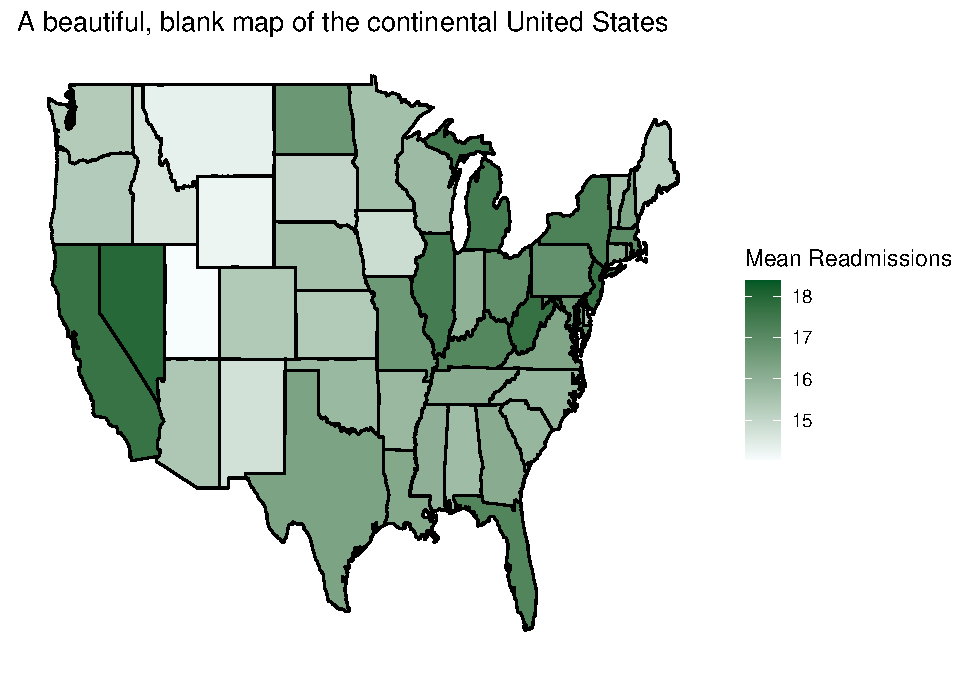
\includegraphics{Demo3_files/figure-latex/unnamed-chunk-7-1.pdf}

\texttt{zipcodeR} is an incredibly handy package when working with US
data! The \texttt{search\_state()} function will look up an abbreviation
and return a state name for us.

\begin{Shaded}
\begin{Highlighting}[]
\CommentTok{\# search\_state(pneumoniaFull$State)}
\end{Highlighting}
\end{Shaded}


\end{document}
